\chapter{Delft3D Model}
\label{chap:Delft3DModel}
This chapter describes the simulations that were made using Delft3D software from Deltares. The input parameters are discussed, as well as the process of setting up the model and the output related to previously found behaviour of the Paraná Guazú. 

\section{Two-dimensional hydrodynamic model}
First, the hydrodynamic conditions of the study area are simulated by setting up a 2D model. For this purpose, the Delft3D 4 Suite version is applied. This software uses structured grids in which the geometry of the cells is fixed. The two-dimensional approach implies that for every cell, depth-averaged flow conditions govern. It is possible to expand to a 3D model by defining sub-layers over the depth profile. For the sake of simplicity, and the level of detail needed in this study, the 2D model is considered sufficient here. 

\subsection{Grid and bathymetry definition}
\label{section:bathemetry}
The grid is defined similar to Figure \ref{fig:cross section domain}, including an extension of the Talabera branch. This ensures reliable computations in the confluence of the Paraná Guazú and Talabera. The \textit{RFRGRID}-tool was applied to generate the grid, after importing land boundaries and manually drawing splines. The grid was then refined twice, using a refinement factor of 3. 

The bathymetry is provided by INA through a Digital Elevation Model from 2019. This was converted to a file containing geospatial information and corresponding depths. The DEM has been visually compared to the ADCP cross sections that result from the field campaign, and it was found that the DEM is representative for the current bathymetry of the river. By making use of the \textit{QUICKIN}-tool, the data is interpolated to the computational grid. The resulting grid and depth file, as shown in Figure \ref{fig:delftgrid} and Figure \ref{fig:depthprofile}, were found by implementing the following operations:

\begin{itemize}
    \item Grid Cell Averaging with 1 as a minimum number of averaging points. This method is preferred over Triangular Interpolation, which is computationally more expensive. In addition, the Grid Cell Averaging approach is suitable when there are more samples than grid points \autocite{deltaresQUICKINUserManual2025}. This is found to be the case when mapping the DEM raster data to a grid. 
    \item Internal Diffusion with 1000 internal diffusion steps. This approach helps building a smooth transition between 'blank' points (no depth value) and existing bathymetry. 
\end{itemize}

Subsequently, the grid and depth profile mark the domain to which the flow input can be assigned. In Section \ref{sec:flow input}, this input is described. 


\begin{figure}[H]
    \centering
    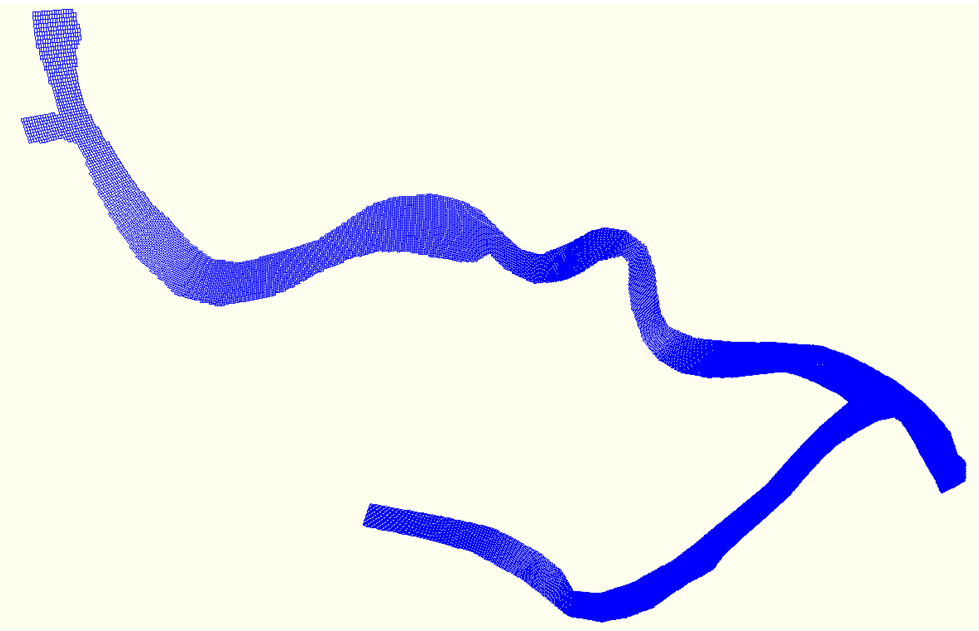
\includegraphics[width=0.5\linewidth]{figures/ch7/delftgrid.PNG}
    \caption{Delft3D grid for 2D hydrodynamic model}
    \label{fig:delftgrid}
\end{figure}

\begin{figure}[H]
    \centering
    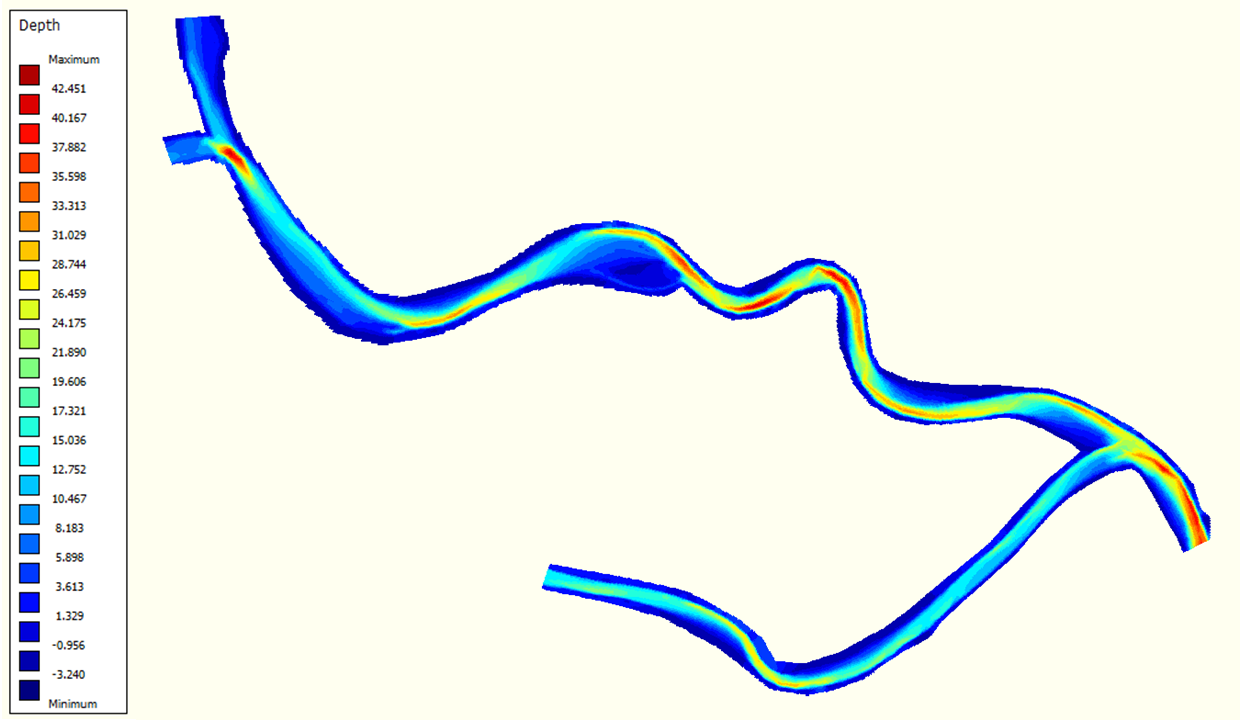
\includegraphics[width=0.5\linewidth]{figures/ch7/depthprofile.PNG}
    \caption{Depth profile for 2D hydrodynamic model made by use of QUICKIN}
    \label{fig:depthprofile}
\end{figure}



\subsection{Input for hydrodynamic simulation (Delft3D-FLOW)}
\label{sec:flow input}
This section discusses the boundary conditions, hydrodynamic input and parameters that are necessary to run the 2D model simulation. The time frame ran from September 24 to September 26, the dates of the fieldwork. In terms of processes included in the model, only secondary flow is considered. The initial conditions are defined by the water level at the downstream boundary (Brazo Largo) at the start time of the simulation, and a zero secondary flow velocity. In addition, boundary conditions and physical parameters have to be defined. The default settings for the numerical parameters are assumed to be applicable. 

\subsubsection{Boundary conditions}
In total, there are four boundaries in the domain. To the downstream boundary in Brazo Largo, a time series of water level measurements is assigned. The time series lasts the three days of the time frame, with a measurement every 20 minutes. The other three boundaries have fluvial discharge time series as boundary conditions. There is no measured data available for this. Therefore, the output of a one-dimensional HEC-RAS model was shared by INA. This included discharge time series during the time frame. 

Using the discharge measurements from the field campaign, assumptions are made of the percentages of the discharge that is divided over the domain. These ratios were derived from Table \ref{tab:discharges fieldwork}. Subsequently, the percentages are multiplied by the Brazo Largo discharge series to find appropriate boundary conditions in the remaining boundaries.

\subsubsection{Physical parameters}
The following physical parameters form the input for the flow model. For other parameters, default settings were applied. 

\begin{itemize}
    \item Adjustment parameter for near-bed velocity for computation of bed shear stress: $\beta_c = 0.5$
    \item Bottom roughness is described by uniform Manning values: $U = V = 0.025$
    \item Uniform value for horizontal eddy viscosity: $1 ~m^2/s$
    \item Uniform value for horizontal eddy diffusivity: $10 ~m^2/s$
\end{itemize}


\subsection{Output of 2D hydrodynamic model}